\chapter{Búsqueda exhaustiva}

La \key{búsqueda exhaustiva}
es un método general que se puede utilizar
para resolver casi cualquier problema algorítmico.
La idea es generar todas las posibles
soluciones al problema mediante fuerza bruta,
y luego seleccionar la mejor solución o contar el
número de soluciones, dependiendo del problema.

La búsqueda exhaustiva es útil
si hay suficiente tiempo para revisar todas las soluciones,
ya que suele ser fácil de implementar
y siempre proporciona la respuesta correcta.
Si la búsqueda exhaustiva es demasiado lenta,
pueden ser necesarias otras técnicas, como algoritmos voraces o
programación dinámica.

\section{Generar subconjuntos}

\index{subconjunto}

Primero consideramos el problema de generar
todos los subconjuntos de un conjunto de $n$ elementos.
Por ejemplo, los subconjuntos de $\{0,1,2\}$ son
$\emptyset$, $\{0\}$, $\{1\}$, $\{2\}$, $\{0,1\}$,
$\{0,2\}$, $\{1,2\}$ y $\{0,1,2\}$.
Hay dos métodos comunes para esto:
realizar una búsqueda recursiva
o aprovechar la representación en bits de los enteros.

\subsubsection{Método 1}

Una forma elegante de recorrer todos los subconjuntos
de un conjunto es utilizando recursión.
La siguiente función \texttt{buscar}
genera los subconjuntos del conjunto
$\{0,\ldots,n-1\}$.
Esta mantiene un vector \texttt{subconj}
que contendrá los elementos de cada subconjunto.
La búsqueda comienza llamando
a la función con $k = 0$.

\begin{lstlisting}
void buscar(int k) {
    if (k == n) {
        // procesar subconjunto
    } else {
        buscar(k + 1);
        subconj.push_back(k);
        buscar(k + 1);
        subconj.pop_back();
    }
}
\end{lstlisting}

Cuando se llama a la función \texttt{buscar}
con el parámetro $k$,
decide si incluir o no el
elemento de índice $k$ en el subconjunto
y, en ambos casos,
luego se llama a sí misma con el parámetro $k+1$.
Sin embargo, si $k=n$, la función se da cuenta de que
todos los elementos han sido procesados
y se ha generado un subconjunto.

El siguiente árbol ilustra las llamadas a la función cuando $n=3$.
Siempre podemos elegir la rama izquierda
($k$ \emph{no} se incluye en el subconjunto) o la rama derecha
($k$ \emph{sí} se incluye en el subconjunto).

\begin{center}
  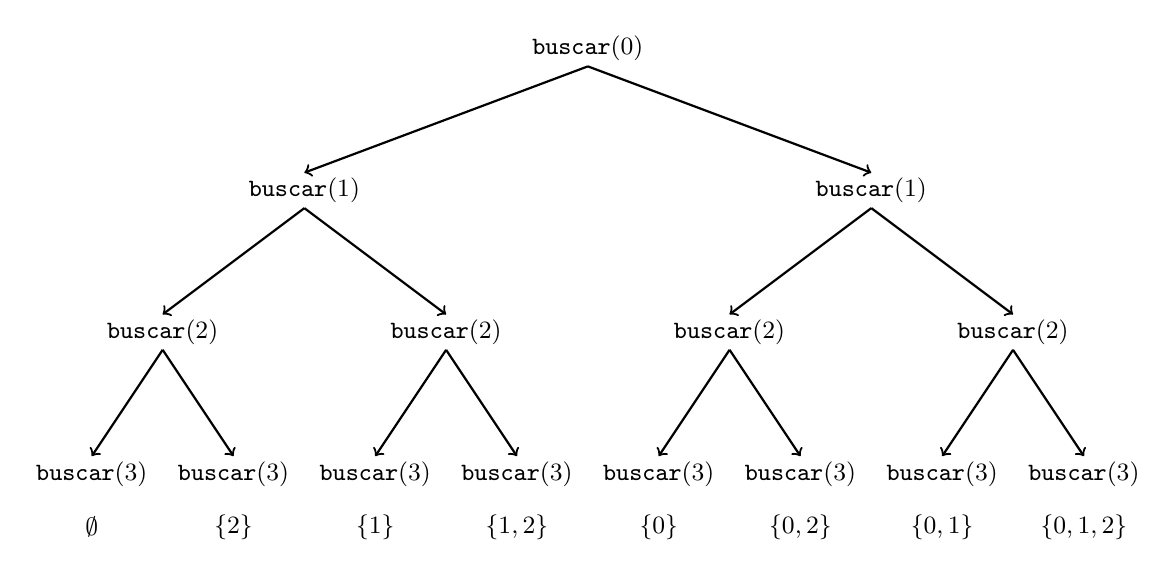
\begin{tikzpicture}[scale=.45]
    \begin{scope}
      \small
      \node at (0,0) {$\texttt{buscar}(0)$};

      \node at (-8,-4) {$\texttt{buscar}(1)$};
      \node at (8,-4) {$\texttt{buscar}(1)$};

      \path[draw,thick,->] (0,0-0.5) -- (-8,-4+0.5);
      \path[draw,thick,->] (0,0-0.5) -- (8,-4+0.5);

      \node at (-12,-8) {$\texttt{buscar}(2)$};
      \node at (-4,-8) {$\texttt{buscar}(2)$};
      \node at (4,-8) {$\texttt{buscar}(2)$};
      \node at (12,-8) {$\texttt{buscar}(2)$};

      \path[draw,thick,->] (-8,-4-0.5) -- (-12,-8+0.5);
      \path[draw,thick,->] (-8,-4-0.5) -- (-4,-8+0.5);
      \path[draw,thick,->] (8,-4-0.5) -- (4,-8+0.5);
      \path[draw,thick,->] (8,-4-0.5) -- (12,-8+0.5);

      \node at (-14,-12) {$\texttt{buscar}(3)$};
      \node at (-10,-12) {$\texttt{buscar}(3)$};
      \node at (-6,-12) {$\texttt{buscar}(3)$};
      \node at (-2,-12) {$\texttt{buscar}(3)$};
      \node at (2,-12) {$\texttt{buscar}(3)$};
      \node at (6,-12) {$\texttt{buscar}(3)$};
      \node at (10,-12) {$\texttt{buscar}(3)$};
      \node at (14,-12) {$\texttt{buscar}(3)$};

      \node at (-14,-13.5) {$\emptyset$};
      \node at (-10,-13.5) {$\{2\}$};
      \node at (-6,-13.5) {$\{1\}$};
      \node at (-2,-13.5) {$\{1,2\}$};
      \node at (2,-13.5) {$\{0\}$};
      \node at (6,-13.5) {$\{0,2\}$};
      \node at (10,-13.5) {$\{0,1\}$};
      \node at (14,-13.5) {$\{0,1,2\}$};


      \path[draw,thick,->] (-12,-8-0.5) -- (-14,-12+0.5);
      \path[draw,thick,->] (-12,-8-0.5) -- (-10,-12+0.5);
      \path[draw,thick,->] (-4,-8-0.5) -- (-6,-12+0.5);
      \path[draw,thick,->] (-4,-8-0.5) -- (-2,-12+0.5);
      \path[draw,thick,->] (4,-8-0.5) -- (2,-12+0.5);
      \path[draw,thick,->] (4,-8-0.5) -- (6,-12+0.5);
      \path[draw,thick,->] (12,-8-0.5) -- (10,-12+0.5);
      \path[draw,thick,->] (12,-8-0.5) -- (14,-12+0.5);
    \end{scope}
  \end{tikzpicture}
\end{center}

\subsubsection{Método 2}

Otra forma de generar subconjuntos se basa en
la representación de bits de los enteros.
Cada subconjunto de un conjunto de $n$ elementos
puede representarse como una secuencia de $n$ bits,
que corresponde a un entero entre $0 \ldots 2^n-1$.
Los unos en la secuencia de bits indican
qué elementos se incluyen en el subconjunto.

La convención habitual es que
el último bit corresponde al elemento 0,
el penúltimo bit corresponde al elemento 1,
y así sucesivamente.
Por ejemplo, la representación de bits de 25
es 11001, que corresponde al subconjunto $\{0,3,4\}$.

El siguiente código recorre los subconjuntos
de un conjunto de $n$ elementos

\begin{lstlisting}
for (int b = 0; b < (1 << n); b++) {
    // procesar subconjunto
}
\end{lstlisting}

El siguiente código muestra cómo podemos encontrar
los elementos de un subconjunto que corresponde a una secuencia de bits.
Al procesar cada subconjunto,
el código construye un vector que contiene los
elementos en el subconjunto.

\begin{lstlisting}
for (int b = 0; b < (1 << n); b++) {
    vector<int> subconj;
    for (int i = 0; i < n; i++) {
        if (b & (1 << i)) subconj.push_back(i);
    }
}
\end{lstlisting}

\section{Generar permutaciones}

\index{permutación}

A continuación, consideramos el problema de generar
todas las permutaciones de un conjunto de $n$ elementos.
Por ejemplo, las permutaciones de $\{0,1,2\}$ son
$(0,1,2)$, $(0,2,1)$, $(1,0,2)$, $(1,2,0)$,
$(2,0,1)$ y $(2,1,0)$.
De nuevo, hay dos métodos:
podemos usar recursión o recorrer las
permutaciones de forma iterativa.

\subsubsection{Método 1}

Al igual que los subconjuntos, las permutaciones se pueden generar
usando recursión.
La siguiente función \texttt{buscar} recorre
las permutaciones del conjunto $\{0,1,\ldots,n-1\}$.
La función construye un vector \texttt{permutaciónm}
que contiene la permutación,
y la búsqueda comienza llamando a la función.

\begin{lstlisting}
void buscar() {
    if (permutación.size() == n) {
        // procesar permutación
    } else {
        for (int i = 0; i < n; i++) {
            if (elegido[i]) continue;
            elegido[i] = true;
            permutación.push_back(i);
            buscar();
            elegido[i] = false;
            permutación.pop_back();
        }
    }
}
\end{lstlisting}

Cada llamada a la función añade un nuevo elemento a
\texttt{permutación}.
El vector \texttt{elegido} indica cuáles
elementos ya están incluidos en la permutación.
Si el tamaño de \texttt{permutación} es igual al tamaño del conjunto,
se ha generado una permutación.

\subsubsection{Método 2}

\index{next\_permutation@\texttt{next\_permutation}}

Un método simple es comenzar con la permutación
$\{0,\ldots,n-1\}$ y usar repetidamente
una función que construye la siguiente permutación
en orden creciente.
La biblioteca estándar de C++ contiene la función
\texttt{next\_permutation} que se puede utilizar para esto:

\begin{lstlisting}
vector<int> permutación; // construir permutación inicial
for (int i = 0; i < n; i++) permutación.push_back(i);

do {
    // procesar permutación
} while (next_permutation(permutación.begin(), permutación.end()));
\end{lstlisting}

\section{Backtracking}

\index{backtracking}

Un algoritmo que utiliza \key{backtracking}
comienza con una solución vacía
y extiende la solución paso a paso.
La búsqueda recursivamente
recorre todas las diferentes formas en que
se puede construir una solución.

\index{problema de las reinas}

Como ejemplo, considera el problema de
calcular el número
de formas en que $n$ reinas pueden ser colocadas en
un tablero de ajedrez $n \times n$ tal que
ninguna reina ataque a otra.
Por ejemplo, cuando $n=4$,
hay dos soluciones posibles:

\begin{center}
  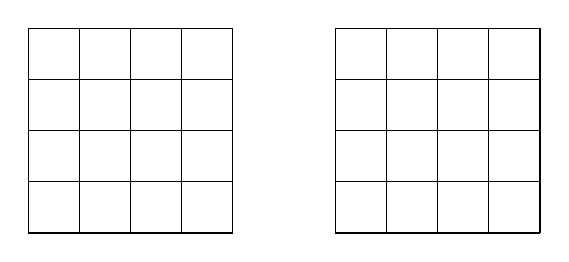
\begin{tikzpicture}[scale=.65]
    \begin{scope}
      \draw (0, 0) grid (4, 4);
      \node at (1.5,3.5) {\symqueen};
      \node at (3.5,2.5) {\symqueen};
      \node at (0.5,1.5) {\symqueen};
      \node at (2.5,0.5) {\symqueen};

      \draw (6, 0) grid (10, 4);
      \node at (6+2.5,3.5) {\symqueen};
      \node at (6+0.5,2.5) {\symqueen};
      \node at (6+3.5,1.5) {\symqueen};
      \node at (6+1.5,0.5) {\symqueen};

    \end{scope}
  \end{tikzpicture}
\end{center}

El problema se puede resolver mediante backtracking
colocando reinas en el tablero fila por fila.
Más precisamente, se colocará exactamente una reina por fila
tal que ninguna reina ataque a otra colocada anteriormente.
Se ha encontrado una solución cuando todas
las $n$ reinas han sido colocadas en el tablero.

Por ejemplo, cuando $n=4$,
algunas soluciones parciales generadas por
el algoritmo de backtracking son las siguientes:

\begin{center}
  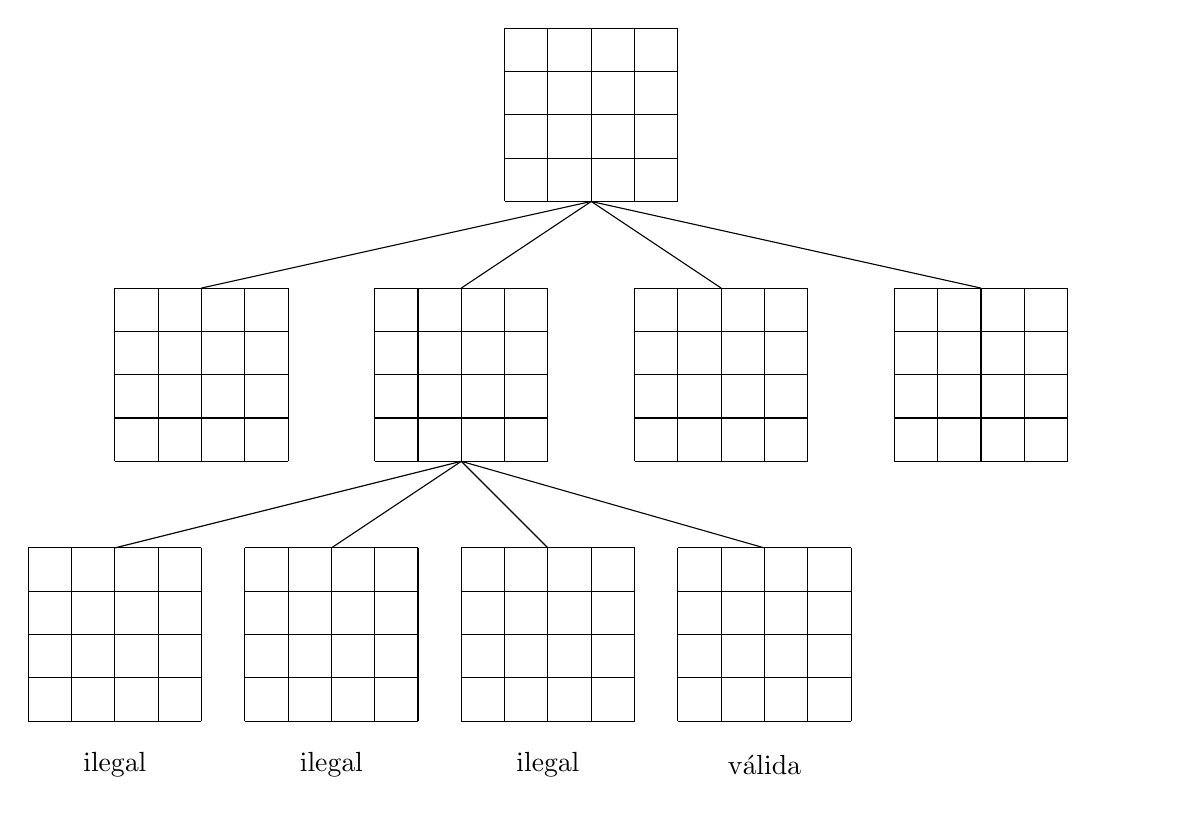
\begin{tikzpicture}[scale=.55]
    \begin{scope}
      \draw (0, 0) grid (4, 4);

      \draw (-9, -6) grid (-5, -2);
      \draw (-3, -6) grid (1, -2);
      \draw (3, -6) grid (7, -2);
      \draw (9, -6) grid (13, -2);

      \node at (-9+0.5,-3+0.5) {\symqueen};
      \node at (-3+1+0.5,-3+0.5) {\symqueen};
      \node at (3+2+0.5,-3+0.5) {\symqueen};
      \node at (9+3+0.5,-3+0.5) {\symqueen};

      \draw (2,0) -- (-7,-2);
      \draw (2,0) -- (-1,-2);
      \draw (2,0) -- (5,-2);
      \draw (2,0) -- (11,-2);

      \draw (-11, -12) grid (-7, -8);
      \draw (-6, -12) grid (-2, -8);
      \draw (-1, -12) grid (3, -8);
      \draw (4, -12) grid (8, -8);
      \draw[white] (11, -12) grid (15, -8);
      \node at (-11+1+0.5,-9+0.5) {\symqueen};
      \node at (-6+1+0.5,-9+0.5) {\symqueen};
      \node at (-1+1+0.5,-9+0.5) {\symqueen};
      \node at (4+1+0.5,-9+0.5) {\symqueen};
      \node at (-11+0+0.5,-10+0.5) {\symqueen};
      \node at (-6+1+0.5,-10+0.5) {\symqueen};
      \node at (-1+2+0.5,-10+0.5) {\symqueen};
      \node at (4+3+0.5,-10+0.5) {\symqueen};

      \draw (-1,-6) -- (-9,-8);
      \draw (-1,-6) -- (-4,-8);
      \draw (-1,-6) -- (1,-8);
      \draw (-1,-6) -- (6,-8);

      \node at (-9,-13) {ilegal};
      \node at (-4,-13) {ilegal};
      \node at (1,-13) {ilegal};
      \node at (6,-13) {válida};

    \end{scope}
  \end{tikzpicture}
\end{center}

En el nivel más bajo, las tres primeras configuraciones
son ilegales, porque las reinas se atacan entre sí.
Sin embargo, la cuarta configuración es válida
y se puede extender a una solución completa colocando
dos reinas más en el tablero.
Solo hay una forma de colocar las dos reinas restantes.

\newpage
El algoritmo se puede implementar de la siguiente manera:
\begin{lstlisting}
void buscar(int y) {
    if (y == n) {
        cuenta++;
        return;
    }
    for (int x = 0; x < n; x++) {
        if (col[x] || diag1[x + y] || diag2[x - y + n - 1]) continue;
        col[x] = diag1[x + y] = diag2[x - y + n - 1] = true;
        search(y + 1);
        col[x] = diag1[x + y] = diag2[x - y + n - 1] = false;
    }
}
\end{lstlisting}
La búsqueda comienza llamando la función con $y = 0$.
El tamaño del tablero es de $n \times n$,
y el código calcula el número de soluciones
en \texttt{cuenta}.

El código asume que las filas y columnas
del tablero están numeradas de 0 a $n-1$.
Cuando se llama a la función \texttt{buscar} con el parámetro $y$,
esta coloca una reina en la fila $y$
y luego se llama a sí misma con el parámetro $y+1$.
Finalmente, si $y=n$, se ha encontrado una solución
y la variable \texttt{cuenta} se incrementa en uno.

El arreglo \texttt{col} lleva un registro de las columnas
que contienen una reina,
y los arreglos \texttt{diag1} y \texttt{diag2}
llevan un registro de las diagonales.
No está permitido agregar otra reina a una
columna o diagonal que ya contiene una reina.
Por ejemplo, las columnas y diagonales del
tablero de $4 \times 4$ están numeradas de la siguiente manera:

\begin{center}
  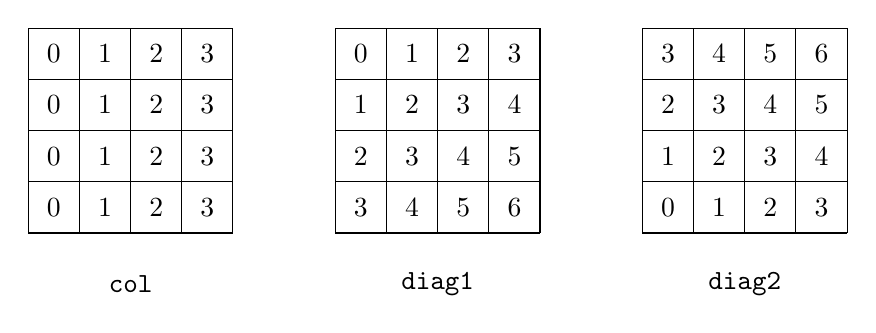
\begin{tikzpicture}[scale=.65]
    \begin{scope}
      \draw (0-6, 0) grid (4-6, 4);
      \node at (-6+0.5,3.5) {$0$};
      \node at (-6+1.5,3.5) {$1$};
      \node at (-6+2.5,3.5) {$2$};
      \node at (-6+3.5,3.5) {$3$};
      \node at (-6+0.5,2.5) {$0$};
      \node at (-6+1.5,2.5) {$1$};
      \node at (-6+2.5,2.5) {$2$};
      \node at (-6+3.5,2.5) {$3$};
      \node at (-6+0.5,1.5) {$0$};
      \node at (-6+1.5,1.5) {$1$};
      \node at (-6+2.5,1.5) {$2$};
      \node at (-6+3.5,1.5) {$3$};
      \node at (-6+0.5,0.5) {$0$};
      \node at (-6+1.5,0.5) {$1$};
      \node at (-6+2.5,0.5) {$2$};
      \node at (-6+3.5,0.5) {$3$};

      \draw (0, 0) grid (4, 4);
      \node at (0.5,3.5) {$0$};
      \node at (1.5,3.5) {$1$};
      \node at (2.5,3.5) {$2$};
      \node at (3.5,3.5) {$3$};
      \node at (0.5,2.5) {$1$};
      \node at (1.5,2.5) {$2$};
      \node at (2.5,2.5) {$3$};
      \node at (3.5,2.5) {$4$};
      \node at (0.5,1.5) {$2$};
      \node at (1.5,1.5) {$3$};
      \node at (2.5,1.5) {$4$};
      \node at (3.5,1.5) {$5$};
      \node at (0.5,0.5) {$3$};
      \node at (1.5,0.5) {$4$};
      \node at (2.5,0.5) {$5$};
      \node at (3.5,0.5) {$6$};

      \draw (6, 0) grid (10, 4);
      \node at (6.5,3.5) {$3$};
      \node at (7.5,3.5) {$4$};
      \node at (8.5,3.5) {$5$};
      \node at (9.5,3.5) {$6$};
      \node at (6.5,2.5) {$2$};
      \node at (7.5,2.5) {$3$};
      \node at (8.5,2.5) {$4$};
      \node at (9.5,2.5) {$5$};
      \node at (6.5,1.5) {$1$};
      \node at (7.5,1.5) {$2$};
      \node at (8.5,1.5) {$3$};
      \node at (9.5,1.5) {$4$};
      \node at (6.5,0.5) {$0$};
      \node at (7.5,0.5) {$1$};
      \node at (8.5,0.5) {$2$};
      \node at (9.5,0.5) {$3$};

      \node at (-4,-1) {\texttt{col}};
      \node at (2,-1) {\texttt{diag1}};
      \node at (8,-1) {\texttt{diag2}};

    \end{scope}
  \end{tikzpicture}
\end{center}

Sea $q(n)$ el número de formas de
colocar $n$ reinas en un tablero de ajedrez de $n \times n$.
El algoritmo de backtracking anterior nos dice que, por ejemplo, $q(8)=92$.
Cuando $n$ aumenta, la búsqueda se vuelve rápidamente lenta,
porque el número de soluciones aumenta
exponencialmente.
Por ejemplo, calcular $q(16)=14772512$
usando el algoritmo anterior ya toma aproximadamente un minuto
en una computadora moderna.\footnote{No se conoce ninguna forma eficiente de
  calcular valores más grandes de $q(n)$. El récord actual es
  $q(27)=234907967154122528$, calculado en 2016 \cite{q27}.}

\newpage
\section{Podar la búsqueda}

A menudo podemos optimizar backtracking \emph{podando} el árbol de búsqueda.
La idea es agregar ``inteligencia'' al algoritmo
para que pueda notar lo antes posible
si una solución parcial no puede extenderse
a una solución completa.
Dichas optimizaciones pueden tener un tremendo
efecto en la eficiencia de la búsqueda.

Consideremos el problema
de calcular el número de caminos
en una cuadrícula de $n \times n$ desde la esquina superior izquierda
hasta la esquina inferior derecha, de tal manera que
el camino visite cada cuadrado exactamente una vez.
Por ejemplo, en una cuadrícula de $7 \times 7$,
hay 111.712 de estos caminos.
Uno de los caminos es el siguiente:

\begin{center}
  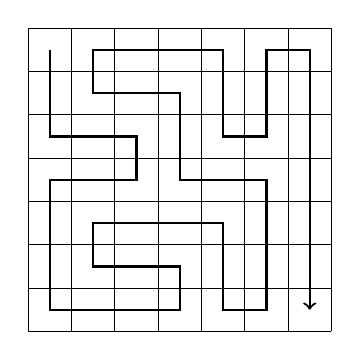
\begin{tikzpicture}[scale=.55]
    \begin{scope}
      \draw (0, 0) grid (7, 7);
      \draw[thick,->] (0.5,6.5) -- (0.5,4.5) -- (2.5,4.5) --
      (2.5,3.5) -- (0.5,3.5) -- (0.5,0.5) --
      (3.5,0.5) -- (3.5,1.5) -- (1.5,1.5) --
      (1.5,2.5) -- (4.5,2.5) -- (4.5,0.5) --
      (5.5,0.5) -- (5.5,3.5) -- (3.5,3.5) --
      (3.5,5.5) -- (1.5,5.5) -- (1.5,6.5) --
      (4.5,6.5) -- (4.5,4.5) -- (5.5,4.5) --
      (5.5,6.5) -- (6.5,6.5) -- (6.5,0.5);
    \end{scope}
  \end{tikzpicture}
\end{center}

Nos enfocamos en el caso de $7 \times 7$,
porque su nivel de dificultad es apropiado para nuestras necesidades.
Comenzaremos con un algoritmo de backtracking sencillo,
y luego lo optimizaremos paso a paso utilizando observaciones
sobre cómo se puede podar la búsqueda.
Después de cada optimización, mediremos el tiempo de ejecución
del algoritmo y el número de llamadas recursivas,
para ver claramente el efecto de cada
optimización en la eficiencia de la búsqueda.

\subsubsection{Algoritmo básico}

La primera versión del algoritmo no contiene optimizaciones.
Simplemente usamos backtracking para generar
todos los caminos posibles desde la esquina superior izquierda hasta
la inferior derecha y los contamos.

\begin{itemize}[itemsep=0em,topsep=0.5em]
  \item tiempo de ejecución: 483 segundos
  \item número de llamadas recursivas: 76 mil millones
\end{itemize}

\subsubsection{Optimización 1}

En cualquier solución, primero avanzamos un paso
hacia abajo o hacia la derecha.
Siempre hay dos caminos que son simétricos
sobre la diagonal de la cuadrícula
después del primer paso.
Por ejemplo, los siguientes caminos son simétricos:

\begin{center}
  \begin{tabular}{ccc}
    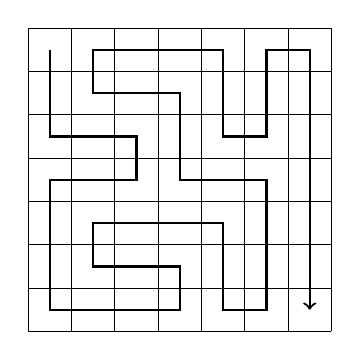
\begin{tikzpicture}[scale=.55]
      \begin{scope}
        \draw (0, 0) grid (7, 7);
        \draw[thick,->] (0.5,6.5) -- (0.5,4.5) -- (2.5,4.5) --
        (2.5,3.5) -- (0.5,3.5) -- (0.5,0.5) --
        (3.5,0.5) -- (3.5,1.5) -- (1.5,1.5) --
        (1.5,2.5) -- (4.5,2.5) -- (4.5,0.5) --
        (5.5,0.5) -- (5.5,3.5) -- (3.5,3.5) --
        (3.5,5.5) -- (1.5,5.5) -- (1.5,6.5) --
        (4.5,6.5) -- (4.5,4.5) -- (5.5,4.5) --
        (5.5,6.5) -- (6.5,6.5) -- (6.5,0.5);
      \end{scope}
    \end{tikzpicture}
     & \hspace{20px}
     &
    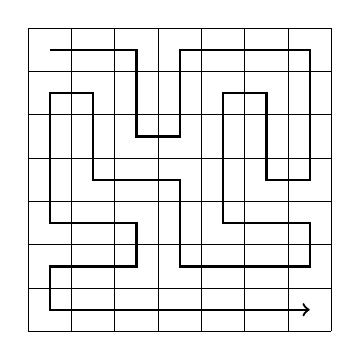
\begin{tikzpicture}[scale=.55]
      \begin{scope}[yscale=1,xscale=-1,rotate=-90]
        \draw (0, 0) grid (7, 7);
        \draw[thick,->] (0.5,6.5) -- (0.5,4.5) -- (2.5,4.5) --
        (2.5,3.5) -- (0.5,3.5) -- (0.5,0.5) --
        (3.5,0.5) -- (3.5,1.5) -- (1.5,1.5) --
        (1.5,2.5) -- (4.5,2.5) -- (4.5,0.5) --
        (5.5,0.5) -- (5.5,3.5) -- (3.5,3.5) --
        (3.5,5.5) -- (1.5,5.5) -- (1.5,6.5) --
        (4.5,6.5) -- (4.5,4.5) -- (5.5,4.5) --
        (5.5,6.5) -- (6.5,6.5) -- (6.5,0.5);
      \end{scope}
    \end{tikzpicture}
  \end{tabular}
\end{center}

Por lo tanto, podemos decidir que siempre primero
nos movemos hacia abajo (o hacia la derecha),
y finalmente multiplicamos el número de soluciones por dos.

\begin{itemize}[itemsep=0em,topsep=0.5em]
  \item tiempo de ejecución: 244 segundos
  \item número de llamadas recursivas: 38 mil millones
\end{itemize}

\subsubsection{Optimización 2}

Si el camino llega a la casilla inferior derecha
antes de haber visitado todas las demás casillas de la cuadrícula,
está claro que
no será posible completar la solución.
Un ejemplo de esto es el siguiente camino:

\begin{center}
  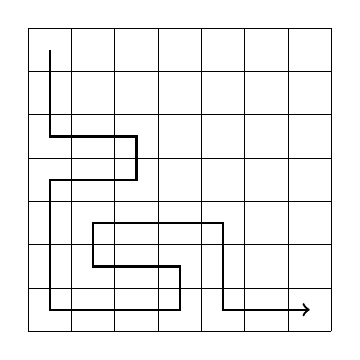
\begin{tikzpicture}[scale=.55]
    \begin{scope}
      \draw (0, 0) grid (7, 7);
      \draw[thick,->] (0.5,6.5) -- (0.5,4.5) -- (2.5,4.5) --
      (2.5,3.5) -- (0.5,3.5) -- (0.5,0.5) --
      (3.5,0.5) -- (3.5,1.5) -- (1.5,1.5) --
      (1.5,2.5) -- (4.5,2.5) -- (4.5,0.5) --
      (6.5,0.5);
    \end{scope}
  \end{tikzpicture}
\end{center}
Usando esta observación, podemos terminar la búsqueda
inmediatamente si llegamos a la casilla inferior derecha demasiado pronto.

\begin{itemize}[itemsep=0em,topsep=0.5em]
  \item tiempo de ejecución: 119 segundos
  \item número de llamadas recursivas: 20 mil millones
\end{itemize}

\subsubsection{Optimización 3}

Si el camino toca una pared
y puede girar hacia la izquierda o hacia la derecha,
la cuadrícula se divide en dos partes
que contienen casillas no visitadas.
Por ejemplo, en la siguiente situación,
el camino puede girar hacia la izquierda o hacia la derecha:

\begin{center}
  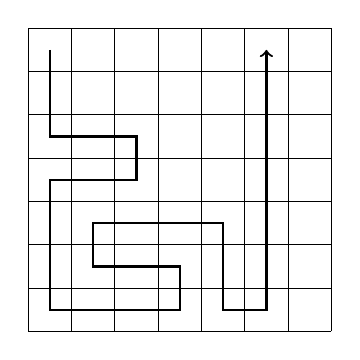
\begin{tikzpicture}[scale=.55]
    \begin{scope}
      \draw (0, 0) grid (7, 7);
      \draw[thick,->] (0.5,6.5) -- (0.5,4.5) -- (2.5,4.5) --
      (2.5,3.5) -- (0.5,3.5) -- (0.5,0.5) --
      (3.5,0.5) -- (3.5,1.5) -- (1.5,1.5) --
      (1.5,2.5) -- (4.5,2.5) -- (4.5,0.5) --
      (5.5,0.5) -- (5.5,6.5);
    \end{scope}
  \end{tikzpicture}
\end{center}
En este caso, ya no podemos visitar todas las casillas,
por lo que podemos terminar la búsqueda.
Esta optimización es muy útil:

\begin{itemize}[itemsep=0em,topsep=0.5em]
  \item tiempo de ejecución: 1,8 segundos
  \item número de llamadas recursivas: 221 millones
\end{itemize}

\subsubsection{Optimización 4}

La idea de la Optimización 3
se puede generalizar:
si el camino no puede continuar hacia adelante
pero puede girar hacia la izquierda o hacia la derecha,
la cuadrícula se divide en dos partes
que contienen casillas no visitadas en ambas partes.
Por ejemplo, considera el siguiente camino:

\begin{center}
  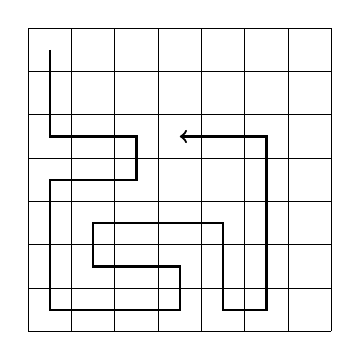
\begin{tikzpicture}[scale=.55]
    \begin{scope}
      \draw (0, 0) grid (7, 7);
      \draw[thick,->] (0.5,6.5) -- (0.5,4.5) -- (2.5,4.5) --
      (2.5,3.5) -- (0.5,3.5) -- (0.5,0.5) --
      (3.5,0.5) -- (3.5,1.5) -- (1.5,1.5) --
      (1.5,2.5) -- (4.5,2.5) -- (4.5,0.5) --
      (5.5,0.5) -- (5.5,4.5) -- (3.5,4.5);
    \end{scope}
  \end{tikzpicture}
\end{center}
Está claro que ya no podemos visitar todas las casillas,
por lo que podemos terminar la búsqueda.
Después de esta optimización, la búsqueda es
muy eficiente:

\begin{itemize}[itemsep=0em,topsep=0.5em]
  \item tiempo de ejecución: 0,6 segundos
  \item número de llamadas recursivas: 69 millones
\end{itemize}

~\\
Ahora es un buen momento para dejar de optimizar
el algoritmo y ver lo que hemos logrado.
El tiempo de ejecución del algoritmo original
era de 483 segundos,
y ahora después de las optimizaciones,
el tiempo de ejecución es de solo 0.6 segundos.
Por lo tanto, el algoritmo se volvió casi 1000 veces
más rápido después de las optimizaciones.

Este es un fenómeno común en backtracking,
porque el árbol de búsqueda suele ser grande
y incluso observaciones simples pueden podar efectivamente
la búsqueda.
Son especialmente útiles las optimizaciones que
ocurren durante los primeros pasos del algoritmo,
es decir, en la parte superior del árbol de búsqueda.

\section{Encuentro en el medio}

\index{encuentro en el medio}

\key{Encuentro en el medio} es una técnica
donde el espacio de búsqueda se divide en
dos partes de aproximadamente igual tamaño.
Se realiza una búsqueda separada
para ambas partes,
y finalmente los resultados de las búsquedas se combinan.

La técnica se puede utilizar
si hay una forma eficiente de combinar los
resultados de las búsquedas.
En tal situación, las dos búsquedas pueden requerir menos
tiempo que una búsqueda grande.
Típicamente, podemos convertir un factor de $2^n$
en un factor de $2^{n/2}$ usando la técnica de encuentro en el
medio.

Como ejemplo, considera un problema donde
se nos da una lista de $n$ números y
un número $x$,
y queremos averiguar si es posible
elegir algunos números de la lista de modo que
su suma sea $x$.
Por ejemplo, dada la lista $[2,4,5,9]$ y $x=15$,
podemos elegir los números $[2,4,9]$ para obtener $2+4+9=15$.
Sin embargo, si $x=10$ para la misma lista,
no es posible formar la suma.

Un algoritmo simple para el problema es recorrer
todos los subconjuntos de los elementos y
verificar si la suma de alguno de los subconjuntos es $x$.
El tiempo de ejecución de dicho algoritmo es $O(2^n)$,
porque hay $2^n$ subconjuntos.
Sin embargo, usando la técnica de encuentro en el medio,
podemos lograr un algoritmo más eficiente de tiempo $O(2^{n/2})$.
\footnote{Esta idea fue introducida en 1974 por E. Horowitz y
  S. Sahni \cite{hor74}.}
Ten en cuenta que $O(2^n)$ y $O(2^{n/2})$ son diferentes
complejidades porque $2^{n/2}$ es igual a $\sqrt{2^n}$.

La idea es dividir la lista en
dos sublistas $A$ y $B$ de modo que ambas
contengan aproximadamente la mitad de los números.
La primera búsqueda genera todos los subconjuntos
de $A$ y almacena sus sumas en una lista $S_A$.
Correspondientemente, la segunda búsqueda crea
una lista $S_B$ a partir de $B$.
Después de esto, basta con verificar si es posible
elegir un elemento de $S_A$ y otro
elemento de $S_B$ de modo que su suma sea $x$.
Esto es posible exactamente cuando hay una forma de
formar la suma $x$ usando los números de la lista original.

Por ejemplo, suponga que la lista es $[2,4,5,9]$ y $x=15$.
Primero, dividimos la lista en $A=[2,4]$ y $B=[5,9]$.
Luego, creamos las listas
$S_A=[0,2,4,6]$ y $S_B=[0,5,9,14]$.
En este caso, la suma $x=15$ es posible de formar,
porque $S_A$ contiene la suma $6$,
$S_B$ contiene la suma $9$, y $6+9=15$.
Esto corresponde a la solución $[2,4,9]$.

Podemos implementar el algoritmo de manera que
su complejidad de tiempo sea $O(2^{n/2})$.
Primero, generamos listas \emph{ordenadas} $S_A$ y $S_B$,
lo cual se puede hacer en tiempo $O(2^{n/2})$ utilizando una técnica similar al merge.
Después de esto, dado que las listas están ordenadas,
podemos verificar en tiempo $O(2^{n/2})$ si
la suma $x$ se puede crear a partir de $S_A$ y $S_B$.
